\begin{name}
	{\tenchude}
	{\tendethi}
	{\tentruong}
	{\thoigian}
\end{name}
\setcounter{ex}{0}\setcounter{bt}{0}
\begin{ex}%[1H4H4-2]
	\immini{Cho hình chóp $S. ABCD$. Gọi $M$, $N$, $P$ lần lượt là trung điểm các cạnh $SA$, $AB$ và $AD$ (tham khảo hình bên).
		Mặt phẳng $\left(MNP\right)$ song song với mặt phẳng nào dưới đây?
		\choice
		{\True $\left(SBD\right)$}
		{$\left(SCD\right)$}
		{$\left(ABCD\right)$}
		{$\left(SBC\right)$}}
	{
		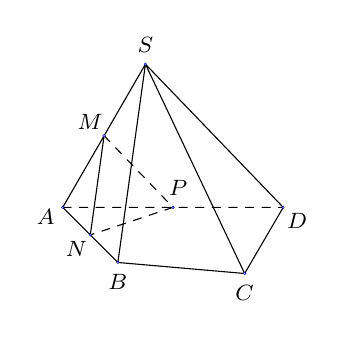
\begin{tikzpicture}[xscale=0.7,yscale=0.7,>=stealth, font=\footnotesize, line join=round, line cap=round,declare function={h=3;}]
			\path
			(0,0) coordinate (A)
			(1,-1) coordinate (B)
			(3.3,-1.2) coordinate (C)
			(4,0) coordinate (D)
			(A)+(60:h) coordinate (S)
			(barycentric cs:A=1,S=1)coordinate(M)
			(barycentric cs:A=1,B=1)coordinate(N)
			(barycentric cs:A=1,D=1)coordinate(P)
			;
			\draw[dashed] (M)--(P)--(N) (A)--(D);
			\draw (C)--(S)--(A)--(B)--(C)--(D)--(S)--(B) (M)--(N);
			\foreach \p/\g in{A/-150,B/-90,C/-90,D/-45,S/90,M/135,N/-135,P/75}
			\shade[shading=ball](\p)circle(.03)node[shift={(\g:.25)},scale=1]{$\p$};
		\end{tikzpicture}
	}
	\loigiai{
		Ta có $MP\parallel SD;MP\not\subset\left(SBD\right)$ $\Rightarrow$ $MP\parallel \left(SBD\right)$.\\
		$MN\parallel SB;MN\not\subset\left(SBD\right)$ $\Rightarrow$ $MN\parallel \left(SBD\right)$\\
		$MN$ cắt $MP$ trong $\left(MNP\right)$\\
		Từ đó suy ra $\left(MNP\right)\parallel \left(SBD\right)$.
	}
\end{ex}

\begin{ex}%[1H4H1-3]
	Cho hình chóp tứ giác $S.ABCD$ và $M$ là một điểm thuộc cạnh $SC$ ($M$ khác $S$ và $C$). Giả sử hai đường thẳng $AB$ cà $CD$ cắt nhau tại $N$. Giao tuyến của hai mặt phẳng $\left(ABM\right)$ và $\left(SCD\right)$ cắt đường thẳng nào trong các đường thẳng sau
	\choice
	{\True $SD$}
	{$SA$}
	{$AD$}
	{$AC$}
	\loigiai{
		\immini{$M$ là điểm chung thứ nhất của hai mặt phẳng $\left(ABM\right)$ và $\left(SCD\right).\quad (1)$\\
			Do $AB$ và $CD$ cắt nhau tại $N$ nên \\
			$N\in AB\subset\left(ABM\right)\Rightarrow N\in \left(ABM\right);\\
				N\in CD\subset\left(SDC\right)\Rightarrow N\in \left(SDC\right)$.\\
			Vậy $N$ là điểm chung thứ hai của hai mặt phẳng $\left(ABM\right)$ và $\left(SCD\right).\quad(2)$\\
			Từ $(1)$ và $(2)$ ta có $MN$ là giao tuyến của hai mặt phẳng $\left(ABM\right)$ và $\left(SCD\right)$.\\
			$MN$ cắt $SD$ trong mặt phẳng $SCD$.}
		{\begin{tikzpicture}[>=stealth,line join=round,line cap=round,font=\footnotesize,scale=0.7]
				\path
				(2,6) coordinate (S)
				(-2,0) coordinate (A)
				(7,0) coordinate (D)
				(0,-3) coordinate (N)
				($(D)!0.4!(N)$) coordinate (C)
				($(A)!0.6!(N)$) coordinate (B)
				($(S)!0.6!(C)$) coordinate (M)
				(intersection of M--N and S--D) coordinate (K)
				;
				\draw[dashed] (M)--(A)--(D) (B)--(C);
				\draw (S)--(A)--(N)--(D)--cycle (N)--(K) (M)--(B)--(S)--(C);
				\foreach \d/\g in {S/90, B/-150,A/180,C/-45,D/0,M/-20,K/30,N/-90} \fill (\d) circle(1pt) + (\g:.4) node{$\d$};
			\end{tikzpicture}}
	}
\end{ex}
\begin{ex} %[1D3H2-2]
	${\mathop{\lim}\limits_{x\to-2}} \left(2x^2+1\right)$ bằng

	\choice{\True $9$}
	{$5$}
	{$-7$}
	{$+\infty$}
	\loigiai{
		Ta có ${\mathop{\lim}\limits_{x\to-2}} \left(2x^2+1\right)=2\left(-2\right)^2+1=9$.
	}
\end{ex}

\begin{ex}%[1D2H3-3]
	Cho cấp số nhân $2,4,8,\ldots$ Số hạng tổng quát của cấp số nhân đã cho là
	\choice
	{$u_{n}=2^{n+1}$}
	{$u_{n}=4^{n}$}
	{\True $u_{n}=2^{n}$}
	{$u_{n}=2^{n-1}$}
		\loigiai{
		Số hạng tổng quát của CSN: $u_{n}=u_{1} \cdot q^{n-1}=2 \cdot 2^{n-1}=2^{n}$.
		}
\end{ex}

\begin{ex}%[1D3N3-1]
	Hàm số nào sau đây liên tục trên $\mathbb{R}$?
	\choice
	{\True $y=\sqrt{x^2+2023}$}
	{$y=\dfrac{1}{x+2023}$}
	{$y=\tan x$}
	{$y=\sqrt{x-1}$}
	\loigiai{
		Hàm số $y=\sqrt{x^2+2023}$ có tập xác định là $\mathbb{R}$ nên nó liên tục trên $\mathbb{R}$.
	}
\end{ex}

\begin{ex}Cau20%[1H4N3-1]
	Trong không gian có bao nhiêu vị trí tương đối giữa đường thẳng và mặt phẳng?
	\choice
	{$1$}
	{$2$}
	{\True $3$}
	{$4$}
	\loigiai{
		Có ba vị trí tương đối giữa đường thẳng và mặt phẳng.
	}
\end{ex}

\begin{ex}%[1H4N1-3]%[Lê Xuân Hòa ]
	Cho $4$ điểm $A$, $B$, $C$, $D$ không cùng nằm trên mặt phẳng. Trên $AB$, $AD$ lần lượt lấy $2$ điểm $M$, $N$ sao cho $MN$ cắt $BD$ tại $I$. Điểm $I$ không thuộc mặt phẳng nào sau đây?
	\choice
	{$(ABD)$}
	{$(BCD)$}
	{$(CMN)$}
	{\True $(ACD)$}
	\loigiai{
		\immini{Vì $I=MN\cap BD$ nên $I\in\left(ABD\right)$, $I\in\left( BCD\right)$, $I\in\left(CMN\right)$.
		}
		{
			\begin{tikzpicture}[line join=round, line cap=round,thick,scale=0.6]
				\coordinate (A) at (0,4);
				\coordinate (D) at (-4,0);
				\coordinate (B) at (0,-2);
				\coordinate (C) at (3,0);
				\coordinate (M) at  ($(A)!0.3!(B)$);
				\coordinate (N) at  ($(A)!0.6!(D)$);
				\tkzInterLL(B,D)(M,N)
				\tkzGetPoint{I}
				\draw(A)--(D) (A)--(B) (A)--(C) (B)--(C) (D)--(B) (M)--(I) (D)--(I);
				\draw[dashed,thin](D)--(C);
				\tkzLabelPoints[left](I)
				\tkzLabelPoints[above left](N)
				\tkzLabelPoints[right](M, C)
				\tkzLabelPoints[above](A)
				\tkzLabelPoints[below](B,D)
			\end{tikzpicture}
		}
	}
\end{ex}

\begin{ex}%[1D1H4-6]
	Tập giá trị của hàm số $y=5\sin x-12\cos x$ là
	\choice
	{$[-12;5]$}
	{\True $[-13;13]$}
	{$[-17;17]$}
	{$(-13;13)$}
	\loigiai{
		Ta có
		\allowdisplaybreaks
		\begin{eqnarray*}
			y &=& 5\sin x-12\cos x=13\left(\dfrac{5\sin x-12\cos x}{13}\right)\\
			&=& 13\left( \sin \alpha\sin x-\cos \alpha \cos x\right)\\
			&=& -13\cos (x+\alpha).\quad \left(\text{với}\, \sin\alpha=\dfrac{5}{13},\cos \alpha=\dfrac{12}{13}\right)
		\end{eqnarray*}
		Lại có $-1\le \cos (x+\alpha)\le 1\Leftrightarrow -13\le -13\cos (x+\alpha)\le 13$.\\
		Vậy tập giá trị hàm số $y=5\sin x-12\cos x$ là $[-13;13]$.
	}
\end{ex}

\begin{ex}%[BG 11 - Nguyen Huynh]%[1D1H4-3]
	\immini{Cho hàm số $y=2\sin x$ trên đoạn $[-\pi;\pi]$ có đồ thị như hình bên. Xét tính đúng sai của các khẳng định sau:
	\choice
	{\True Tập xác định của hàm số $y=2\sin x$ là $\mathbb{R}$}
	{Tập giá trị của hàm số là $[-1;1]$}
	{Hàm số đồng biến trên khoảng $(-2;2)$}
	{Đồ thị hàm số trên đoạn $[-\pi;\pi]$ cắt đường thẳng $y=-2$ tại đúng 2 điểm phân biệt}
	}
	{\begin{tikzpicture}[scale=0.8,>=stealth, font=\footnotesize, line join=round, line cap=round]
	\def\xmin{-4} \def\xmax{4} \def\ymin{-2.5} \def\ymax{2.8}
	\draw[->] (\xmin,0)--(\xmax,0) node [below]{$x$};
	\draw[->] (0,\ymin)--(0,\ymax) node [right]{$y$};
	\node at (0,0) [below right]{$O$};
	\clip (\xmin+0.1,\ymin+0.1) rectangle (\xmax-0.5,\ymax-0.1);
	\draw[smooth,samples=400,domain=\xmin:\xmax] plot(\x,{2*sin(\x r)});
	\draw[dashed] (\xmin,2)--(\xmax,2) (\xmin,-2)--(\xmax,-2);
	\foreach \x in {-2*pi,-1.5*pi,-pi,-0.5*pi,0}
	{\draw[fill=black] (\x,2*sin \x*180/pi) circle (1pt);
	\draw[dashed] (\x,2*sin \x*180/pi)--(\x,0);
	\draw[fill=black] (-\x,2*sin -\x*180/pi) circle (1pt);
	\draw[dashed] (-\x,2*sin -\x*180/pi)--(-\x,0);}
	\node at (0,2.3) [left]{$2$};
	\node at (0,-2.3) [left]{$-2$};
	\node at (-2*pi+0.15,0) [below]{$-2\pi$};
	\node at (-1.5*pi,0) [below]{$-\frac{3\pi}{2}$};
	\node at (-pi-0.15,0) [below]{$-\pi$};
	\node at (-0.5*pi,0) [above]{$-\frac{\pi}{2}$};
	\node at (0.5*pi,0) [below]{$\frac{\pi}{2}$};
	\node at (pi-0.1,0) [below]{$\pi$};
	\node at (1.5*pi,0) [above]{$\frac{3\pi}{2}$};
	\node at (2*pi+0.2,0) [below]{$2\pi$};
	\end{tikzpicture}}
	\loigiai{Dựa vào đồ thị của hàm số, ta có
	\begin{itemchoice}
	\itemch Đúng.\\
	Tập xác định của hàm số là $\mathbb{R}$.
	\itemch Sai.\\ Tập giá trị của hàm số là $[-2;2]$.
	\itemch Sai.\\ Hàm số đồng biến trên khoảng $\left(\dfrac{-\pi}{2};\dfrac{\pi}{2} \right) $.
	\itemch Sai. \\ Đồ thị hàm số trên đoạn $[-\pi;\pi]$ cắt đường thẳng $y=-2$ tại đúng 2 điểm phân biệt.
	\end{itemchoice}}
	\end{ex}

\begin{ex}%[1D3H1-2]
	Giới hạn $\lim\dfrac{3n-7}{2n^2+3n-1}$ bằng
	\choice
	{$\dfrac{3}{2}$}
	{$3$}
	{\True $0$}
	{$\dfrac{-3}{2}$}
	\loigiai{Ta có $\lim\dfrac{3n-7}{2n^2+3n-1}=\lim\left(\dfrac{1}{n}\cdot\dfrac{3-\dfrac{7}{n}}{2+\dfrac{3}{n}-\dfrac{1}{n^2}}\right)=0$.}
\end{ex}

\begin{ex}%[1D5H1-4]%[Dự án đề kiểm tra Toán 11 HKI NH23-24-Đợt 1- Phạm Phương]%[CTST-Đề số 5]
	%[TH]
	Doanh thu bán hàng trong 20 ngày được lựa chọn ngẫu nhiên của một cửa hàng được ghi lại ở bảng sau (đơn vị: triệu đồng):
	\begin{center}
		\begin{tabular}{|c|c|c|c|c|c|}
			\hline
			Doanh thu & $[5;7)$ & $[7;9)$ & $[9;11)$ & $[11;13)$ & $[13;15)$ \\
			\hline
			Số ngày   & $2$     & $7$     & $7$      & $3$       & $1$       \\
			\hline
		\end{tabular}
	\end{center}
	Tìm mốt của mẫu số liệu ghép nhóm trên.
	\choice
	{$M_o=10{,}6$}
	{$M_o=11{,}6$}
	{\True $M_o=9$}
	{$M_o=10$}
	\loigiai{
	Nhóm chứa mốt của mẫu số liệu trên là nhóm $[7;9)$ hoặc $[9;11)$.
	\begin{enumerate}
		\item [{\bf TH1.}] Xét nhóm $[7;9)$ ta có $u_m=7$, $u_{m+1}=9$, $n_m=7$, $n_{m+1}=7$, $n_{m-1}=2$.\\
		      Mốt của mẫu số liệu ghép nhóm là
		      \allowdisplaybreaks{\begin{eqnarray*}
				      M_o&=&u_m+\dfrac{n_m-n_{m-1}}{\left(n_m-n_{m-1}\right)+\left(n_m-n_{m+1}\right)}\cdot \left(u_{m+1}-u_m\right)\\
				      &=& 7+\dfrac{7-2}{\left(7-2\right)+\left(7-7\right)}\cdot \left(9-7\right)=9.
			      \end{eqnarray*} }
		\item [{\bf TH2.}] Xét nhóm $[9;11)$ ta có $u_m=9$, $u_{m+1}=11$, $n_m=7$, $n_{m+1}=3$, $n_{m-1}=7$.\\
		      Mốt của mẫu số liệu ghép nhóm là
		      \allowdisplaybreaks{\begin{eqnarray*}
				      M_o&=&u_m+\dfrac{n_m-n_{m-1}}{\left(n_m-n_{m-1}\right)+\left(n_m-n_{m+1}\right)}\cdot \left(u_{m+1}-u_m\right)\\
				      &=& 9+\dfrac{7-7}{\left(7-7\right)+\left(7-3\right)}\cdot \left(11-9\right)=9.
			      \end{eqnarray*} }
	\end{enumerate}
	Vậy mốt của mẫu số liệu ghép nhóm trên là $M_o=9$.
	}
\end{ex}

\begin{ex}%[1D1N4-2]%[Dự án đề ôn tập Toán khối 11 HKI NH23-24-Dot 1-Xuan Vy Pham]%[CTST-Đề số 4]
	Tập xác định của hàm số $y= 2 \cos x - 1$ là
	\choice
	{$\mathscr{D}=\mathbb{R} \setminus \left\{ \dfrac{1}{2} \right\}$}
	{\True $\mathscr{D}=\mathbb{R} $}
	{$\mathscr{D}=\mathbb{R} \setminus \left\{ \dfrac{\pi}{2} + k \pi , k \in \mathbb{Z} \right\}$}
	{$\mathscr{D}=\mathbb{R} \setminus \left\{ \pi + k \pi , k \in \mathbb{Z} \right\}$}
	\loigiai{Tập xác định của hàm  $y= 2 \cos x - 1$ là $\mathbb{R}$.}
\end{ex}

\begin{ex}%[1H4N2-2]%[Pj10-1-HK1-NH23-24-TeamTeXHoa-VUNgocHao]
	Trong không gian, cho tứ diện $ABCD$, vị trí tương đối giữa 2 đường thẳng $AC$ và $BD$ là
	\choice
	{song song}
	{trùng nhau}
	{\True chéo nhau}
	{cắt nhau}
	\loigiai{
		Ta có $AC$ và $BD$ là hai đường thẳng chéo nhau.
	}
\end{ex}

\begin{ex}%[1-HK1]%[VN-MT-9, Nguyen Huynh]%[1H4H6-1]
	Qua phép chiếu song song lên mặt phẳng $(P)$, hai đường thẳng chéo nhau $a$ và $b$ có hình chiếu là hai đường thẳng $a'$ và $b'$. Mệnh đề nào sau đây đúng?
	\choice
	{$a'$ và $b'$ luôn luôn cắt nhau} {$a'$ và $b'$ có thể trùng nhau} {$a'$ và $b'$ không thể song song} {\True $a'$ và $b'$có thể cắt nhau hoặc song song với nhau}
	\loigiai{
		Ta có $a'$ và $b'$ có thể cắt nhau hoặc song song với nhau.}
\end{ex}

\begin{ex}%[1H4N4-1]%[Pj10-1-HK1-NH23-24-TeamTeXHoa-VUNgocHao]
	Cho hình lập phương $ABCD.A' B' C' D'$. Chọn khẳng định đúng.
	\choice
	{\True $(ABCD) \parallel \left(A' B' D'\right)$}
	{$\left(A' D' C\right) \parallel(A B C D)$}
	{ $\left(D' C' A\right) \parallel(A B C D)$}
	{$\left(B C C' B'\right) \parallel(A B C D)$}
	\loigiai{
		\begin{center}
			\begin{tikzpicture}[scale=.7,font=\footnotesize, line join=round, line cap=round, >=stealth]
				\tkzDefPoints{0/0/A,-1/-1.2/B,4/0/D}
				\coordinate (C) at ($(B)+(D)-(A)$);
				\coordinate (A') at ($(A)+(0,4)$);
				\coordinate (B') at ($(A')+(B)-(A)$);
				\coordinate (C') at ($(A')+(C)-(A)$);
				\coordinate (D') at ($(A')+(D)-(A)$);
				\draw (A')--(B')--(C')--(D')--(A')
				(B)--(C)--(D)--(D')
				(B)--(B')
				(C)--(C') ;
				\draw[dashed] (B)--(A)--(D)
				(A)--(A') ;
				\foreach \x/\g in {A/180,B/-120,C/-60,D/0,A'/120,B'/180,C'/100,D'/80} \fill[black](\x) circle (1pt) ($(\x)+(\g:4mm)$) node{$\x$};
			\end{tikzpicture}
		\end{center}
		Theo định nghĩa hình lập phương ta được kết quả.
	}
\end{ex}

\begin{ex}%[1D2H2-3]
	Cho dãy số $\left(u_n\right)$ có số hạng tổng quát là $u_{n}=2\cdot3^n$ với $n\in\mathbb{N^*}$. Công thức truy hồi của dãy số đó là
	\choice
	{$\heva{&u_1=6\\&u_n=6u_{n-1},n>1}$}
	{\True $\heva{&u_1=6\\&u_n=3u_{n-1},n>1}$}
	{$\heva{&u_1=3\\&u_n=3u_{n-1},n>1}$}
	{$\heva{&u_1=3\\&u_n=3u_{n-1},n>1}$}
	\loigiai{ Ta có $u_1=2\cdot3^1=6$.\\  $u_{n-1}=2\cdot 3^{n-1}\Rightarrow3u_{n-1}=2\cdot 3^{n}=u_n$.}
\end{ex}

\begin{ex}%[1D1N3-1]
	Mệnh đề nào dưới đây đúng với mọi $a$, $b$?
	\choice
	{$\cos{\left(a - b \right)} = \sin{a} \sin{b} - \cos{a}\cos{b}$}
	{\True $\cos{\left(a - b \right)} = \cos{a}\cos{b} + \sin{a} \sin{b}$}
	{$\cos{\left(a - b \right)} = \cos{a}\cos{b} - \sin{a} \sin{b}$}
	{$\cos{\left(a - b \right)} = \cos{a}\sin{b} + \sin{a} \cos{b}$}
	\loigiai{
		Ta có $\cos{\left(a - b \right)} = \cos{a}\cos{b} + \sin{a} \sin{b}$.
	}
\end{ex}

\begin{ex}%[1D5N1-2]%[Dự án đề kiểm tra Toán 11 GHKI NH23-24- Nguyễn Cường]%[THPT - Tp HCM]
	Tuổi thọ (năm) của $50$ bình ác quy ô tô được cho như sau
	\begin{center}
		\begin{tabular}{|c|c|c|c|c|c|c|}
			\hline
			Tuổi thọ (năm) & $[2;2{,}5)$ & $[2{,}5;3)$ & $[3;3{,}5)$ & $[3{,}5;4)$ & $[4;4{,}5)$ & $[4{,}5;5)$ \\
			\hline
			Tần số         & $4$         & $9$         & $14$        & $11$        & $7$         & $5$         \\
			\hline
		\end{tabular}
	\end{center}
	Cỡ mẫu của mẫu số liệu ghép nhóm trên là
	\choice
	{\True $50$}
	{$48$}
	{$14$}
	{$6$}
	\loigiai{
		Cỡ mẫu của mẫu số liệu ghép nhóm trên là $n=4+9+14+11+7+5=50$.
	}
\end{ex}

\begin{ex}%[1H4N6-1]
	Phép chiếu song song biến ba đường thẳng song song thành
	\choice
	{ba đường thẳng đôi một song song với nhau}
	{một đường thẳng}
	{thành hai đường thẳng song song}
	{\True cả ba trường hợp trên}
	\loigiai{
		Phép chiếu song song biến ba đường thẳng song song thành ba đường thẳng đôi một song song hoặc một đường thẳng hoặc thành hai đường thẳng song song.
	}
\end{ex}

\begin{ex}%[1D2N3-1]%[Dự án 11 HVA 2024-2025]%[Viết Tường]
	Cho cấp số nhân $(u_n)$ có công bội $q$. Chọn hệ thức đúng trong các hệ thức sau
	\choice
	{$u_k=\sqrt{u_{k+1}\cdot u_{k+2}}$}
	{$u_k=\dfrac{u_{k+1}+u_{k+2}}{2}$}
	{\True $u_k=u_1\cdot q^{k-1}$}
	{$u_k=u_1+(k-1)q$}
	\loigiai
	{
		Công thức số hạng tổng quát của cấp số nhân là $u_k=u_1\cdot q^{k-1}$.
	}
\end{ex}

\begin{ex}%[1D3N1-1]%[Dự án đề ôn tập Toán khối 11 NH23-24-Đợt 1- Bùi Thanh Cương]%[CTST-Đề số 08]
	Cho hai dãy $\left(u_n\right)$ và $\left(v_n\right)$ thỏa mãn $\lim \limits{n \to +\infty}u_n=2$ và $\lim \limits{n \to +\infty}v_n=3.$ Giá trị của $\lim\left(u_n+v_n\right)$ bằng
	\choice
	{$ 6$}
	{\True $ 5$}
	{$-1$}
	{$ 1$}
	\loigiai{
		Ta có $\lim\left(u_n+v_n\right)= \lim \limits{n \to +\infty}u_n+ \lim \limits{n \to +\infty}v_n=2+3=5$.
	}

\end{ex}

\begin{ex}%[1D1N5-1]
	Mệnh đề nào sau đây đúng với mọi $k$ là số nguyên
	\choice
	{\True $\cot{x} = \cot{\alpha} \Leftrightarrow x = \alpha + k \pi$}
	{$\cot{x} = \cot{\alpha} \Leftrightarrow x = \pm \alpha + k \pi$}
	{$\cot{x} = \cot{\alpha} \Leftrightarrow x = \pm \alpha + k2 \pi$}
	{$\cot{x} = \cot{\alpha} \Leftrightarrow x = \pm \alpha + 2k$}
	\loigiai{
		Theo phương trình lượng giác cơ bản ta có $\cot{x} = \cot{\alpha} \Leftrightarrow x = \alpha + k \pi$ với $k \in \mathbb{Z}$.
	}
\end{ex}

\begin{ex}%[1H4H2-2]%[Dự án đề ôn tập Toán Khối 11 HK1 NH23-24-Dot 1-Vương Quốc Phong]%[CTST - Đề số 3]
	Trong không gian, cho hai đường thẳng $a$ và $b$ chéo nhau. Một đường thẳng $c$ song song với $a$. Khẳng định nào sau đây là đúng?
	\choice
	{$b$ và $c$ chéo nhau}
	{$b$ và $c$ cắt nhau}
	{\True $b$ và $c$ chéo nhau hoặc cắt nhau}
	{$b$ và $c$ song song với nhau}
	\loigiai{
		Ta xét lần lượt các phương án
		\begin{itemize}
			\item \lq\lq $b$ và $c$ chéo nhau\rq\rq\ là sai vì $b$, $c$ có thể cắt nhau.
			\item \lq\lq $b$ và $c$ cắt nhau\rq\rq\ là sai vì $b$, $c$ có thể chéo nhau.
			\item \lq\lq $b$ và $c$ song song với nhau\rq\rq\ là sai vì nếu $b$ và $c$ song song thì $a$ và $b$ song song hoặc trùng nhau.
		\end{itemize}
	}
\end{ex}

\begin{ex}%[Pj10-Đề 07 HK1 NH2023-2024 CTST]%[Nguyễn Văn Nay]%[1D3N1-2]
	Tìm giới hạn $\lim \limits{n \to +\infty}\dfrac{3n-1}{2n+1}$.
	\choice
	{$\dfrac{2}{3}$}
	{$3$}
	{$0$}
	{\True $\dfrac{3}{2}$}
	\loigiai{
		Ta có $\lim \limits{n \to +\infty}\dfrac{3n-1}{2n+1}
			=\lim \limits{n \to +\infty}\dfrac{3-\dfrac{1}{n}}{2+\dfrac{1}{n}}
			=\dfrac{\lim \limits{n \to +\infty}\left(3-\dfrac{1}{n} \right)}{\lim \limits{n \to +\infty}\left(2+\dfrac{1}{n} \right)}
			=\dfrac{\lim \limits{n \to +\infty}3-\lim \limits{n \to +\infty}\dfrac{1}{n}}{\lim \limits{n \to +\infty}2+\lim \limits{n \to +\infty}\dfrac{1}{n}}
			=\dfrac{3-0}{2+0}=\dfrac{3}{2}$.
	}
\end{ex}

\begin{ex}%[1H4V1-3]
	Cho hình chóp $S.ABCD$, đáy là tứ giác lồi $ABCD$ có các cạnh đối không song song với nhau. Gọi $M$ là điểm trên cạnh $SA$, $O$ là giao điểm của $AC$ và $BD$. Trong các khẳng định sau, khẳng định nào đúng?
	\choice
	{Giao tuyến của $(SAC)$ và $(SBD)$ là $SM$}
	{\True Giao tuyến của $(SAB)$ và $(SCD)$ là $SF$, với $F$ là giao điểm của $AB$ và $CD$}
	{Giao tuyến của $(SBC)$ và $(SAD)$ là $SM$}
	{Giao tuyến của $(BCM)$ và $(SCD)$ là đường thẳng song song với $SD$}
	\loigiai
	{
		\immini{\begin{itemchoice}
				\itemch Ta có $S\in (SAC)\cap (SBD)$.\quad(1)\\
				Trong mặt phẳng $(ABCD)$, gọi $O=AC\cap BD$.\\
				Suy ra  $O\in (SAC)\cap (SBD)$.\quad(2)\\
				Từ (1) và (2) suy ra $SO= (SAC)\cap (SBD)$.\\
				Vậy giao tuyến của $(SAC)$ và $(SBD)$ là $SO$.
				\itemch Ta có $S\in (SAB)\cap (SCD)$.\quad(3)\\
				Trong mặt phẳng $(ABCD)$, gọi $F=AB\cap CD$.\\
				Suy ra  $F\in (SAB)\cap (SCD)$.\quad(4)\\
				Từ (3) và (4) suy ra $SF= (SAB)\cap (SCD)$.\\
				Vậy giao tuyến của $(SAB)$ và $(SCD)$ là $SF$.
				\itemch Ta có $S\in (SBC)\cap (SAD)$.\quad(5)\\
				Trong mặt phẳng $(ABCD)$, gọi $E=BC\cap AD$.\\
				Suy ra  $E\in (SBC)\cap (SAD)$.\quad(6)\\
				Từ (5) và (6) suy ra $SE= (SBC)\cap (SAD)$.\\
				Vậy giao tuyến của $(SBC)$ và $(SAD)$ là $SE$, không phải $SM$.
				\itemch Ta có $C\in (BCM)\cap (SCD)$.\quad(7)\\
				Trong mặt phẳng $(SAD)$, gọi $G=ME\cap SD$, mà $ME\subset (BCM)$, $SD\subset (SCD)$ nên $G\in (BCM)\cap (SCD)$.\quad(8)\\
				Từ (7) và (8) suy ra $CG=(BCM)\cap(SCD)$.\\
				Ta thấy $CG$ cắt $SD$ trong mặt phẳng $(SCD)$.
			\end{itemchoice}}
		{\begin{tikzpicture}[line cap=round,line join=round,font=\footnotesize]
				\path (0:0) coordinate(A) (0:4) coordinate(D) (-65:2.4) coordinate(B) ++(20:2.3) coordinate(C) (50:3) coordinate(S);
				\path ($(S)!.4!(A)$) coordinate(M) (intersection of A--C and B--D) coordinate(O) (intersection of A--D and B--C) coordinate(E) (intersection of A--B and C--D) coordinate(F);
				\coordinate (G) at (intersection cs:first line={(S)--(D)}, second line={(M)--(E)});
				\coordinate (H) at (intersection cs:first line={(S)--(O)}, second line={(C)--(M)});
				\draw (S)--(A)--(F)--cycle (S)--(C)--(E)--cycle (C)--(F) (S)--(B)--(M);
				\draw[dashed] (S)--(D)--(C)--(A)--(E) (C)--(B)--(D) (S)--(O)--(M)--(C) (M)--(E)(B)--(G)--(C);
				\foreach \d/\g in {A/180, B/-135, C/-45, D/-45, S/90, O/-95, M/150, E/0, F/-90, G/70}
				\fill (\d) circle(1pt) node[shift={(\g:.3)}]{$\d$};
			\end{tikzpicture}}

	}
\end{ex}

\begin{ex}%[1D1H4-7]%[BG K11, Nhật Thiện]
	\immini{Đồ thị trong hình vẽ bên là đồ thị của hàm số nào dưới đây?
		\choice
		{$y=\sin 2x$}
		{$y=2\cos x$}
		{$y=\cos 2x$}
		{\True $y=2\sin x$}
	}
	{\begin{tikzpicture}[scale=0.8,>=stealth, font=\footnotesize, line join=round, line cap=round]
			\def\xmin{-4} \def\xmax{4} \def\ymin{-2.5} \def\ymax{2.8}
			\draw[->] (\xmin,0)--(\xmax,0) node [below]{$x$};
			\draw[->] (0,\ymin)--(0,\ymax) node [right]{$y$};
			\node at (0,0) [below right]{$O$};
			\clip (\xmin+0.1,\ymin+0.1) rectangle (\xmax-0.5,\ymax-0.1);
			\draw[smooth,samples=400,domain=\xmin:\xmax] plot(\x,{2*sin(\x r)});
			\draw[dashed] (\xmin,2)--(\xmax,2) (\xmin,-2)--(\xmax,-2);
			\foreach \x in {-2*pi,-1.5*pi,-pi,-0.5*pi,0}
				{\draw[fill=black] (\x,2*sin \x*180/pi) circle (1pt);
					\draw[dashed] (\x,2*sin \x*180/pi)--(\x,0);
					\draw[fill=black] (-\x,2*sin -\x*180/pi) circle (1pt);
					\draw[dashed] (-\x,2*sin -\x*180/pi)--(-\x,0);}
			\node at (0,2.3) [left]{$2$};
			\node at (0,-2.3) [left]{$-2$};
			\node at (-2*pi+0.15,0) [below]{$-2\pi$};
			\node at (-1.5*pi,0) [below]{$-\frac{3\pi}{2}$};
			\node at (-pi-0.15,0) [below]{$-\pi$};
			\node at (-0.5*pi,0) [above]{$-\frac{\pi}{2}$};
			\node at (0.5*pi,0) [below]{$\frac{\pi}{2}$};
			\node at (pi-0.1,0) [below]{$\pi$};
			\node at (1.5*pi,0) [above]{$\frac{3\pi}{2}$};
			\node at (2*pi+0.2,0) [below]{$2\pi$};
		\end{tikzpicture}}
	\loigiai{
		Từ đồ thị ta thấy hàm số đi qua gốc tọa độ $O(0;0)$, có tung độ cao nhất bằng $2$ và thấp nhất bằng $-2$. Chỉ có hàm số $y=2\sin x$ thỏa mãn.}
\end{ex}

\begin{ex}%[1D5H1-3]%[Dự án đề ôn tập HKI Toán 11 NH23-24- Dương Phước Sang]%[CTST]
	Khảo sát thời gian tập thể dục trong ngày của $1$ số học sinh khối $11$ thu được mẫu số liệu ghép nhóm sau:
	\begin{longtable}{|c|c|c|c|c|c|}
		\hline
		Thời gian (phút) & $[0;20)$ & $[20;40)$ & $[40;60)$ & $[60;80)$ & $[80;100)$ \\
		\hline
		Số học sinh      & $5$      & $9$       & $12$      & $10$      & $6$        \\
		\hline
	\end{longtable}
	Hãy ước lượng thời gian tập thể dục trung bình của một học sinh trong một ngày.
	\choice
	{$53{,}41$}
	{\True $51{,}43$}
	{$38{,}02$}
	{$42{,}83$}
	\loigiai{
		Bảng dữ liệu ghép nhóm có $\overline{x}=\dfrac{10\cdot 5+30\cdot 9+50\cdot 12+70\cdot 10+90\cdot 6}{5+9+12+10+6}=\dfrac{360}{7} \approx 51{,}43$.
	}
\end{ex}

\begin{ex}%[1D2H1-3]
	Cho dãy số $(u_n)$ có $u_1=-3$ và $u_{n+1}=u_n+n$ với $n\ge 1$, $n\in \mathbb{N}$. Số hạng thứ $3$ của dãy số đã cho là
	\choice
	{$u_3=-1$}
	{$u_3=3$}
	{$u_3=-2$}
	{\True $u_3=0$}
	\loigiai{
		Ta có $u_1=-3$ và $u_{n+1}=u_n+n$ với $n\ge 1$, $n\in \mathbb{N}$.\\
		Suy ra $u_2=u_1+1=-3+1=-2$; $u_3=u_2+2=-2+2=0$.
	}
\end{ex}

\begin{ex}%[1D3N2-1]%[Dự án đề kiểm tra Toán 11 HHKI NH23-24- Phạm Văn Long]%[Thi thử - KNTT]
	Cho hai hàm số $f\left(x\right),g\left(x\right)$ thỏa mãn ${\mathop{\lim}\limits_{x\to 2}} f\left(x\right)=5$ và ${\mathop{\lim}\limits_{x\to 2}} g\left(x\right)=1$. Giá trị của ${\mathop{\lim}\limits_{x\to 2}} \left[f\left(x\right)\cdot g\left(x\right)\right]$ bằng
	\choice{\True $5$}
	{$6$}
	{$1$}
	{$-1$}
	\loigiai{
	Ta có ${\mathop{\lim}\limits_{x\to 2}} \left[f\left(x\right)\cdot g\left(x\right)\right]={\mathop{\lim}\limits_{x\to 2}} f\left(x\right)\cdot {\mathop{\lim}\limits_{x\to 2}} g\left(x\right)=5\cdot 1=5$.
		}
\end{ex}

\begin{ex}%[Dự án Giảng K10 - K11]%[Dao-V- Thuy]%[1D2H2-6]
	Cho cấp số cộng $\left(u_n\right)$ xác định bởi $u_n=5n-2$. Biết tổng của $n$ số hạng đầu tiên bằng $2576$, tìm $n$.
	\choice
	{$n=31$}
	{\True $n=32$}
	{$n=33$}
	{$n=34$}
	\loigiai{
		Ta có \[ \dfrac{n(u_1+u_n)}{2}=2576 \Leftrightarrow \dfrac{n(3+5n-2)}{2} =2576 \Leftrightarrow 5n^2+ n-5152=0 \Leftrightarrow \hoac{& n=-\dfrac{161}{5}\\& n= 32.}\]
		Do $n\in \mathbb{N}^*$ nên $n=32$.
	}
\end{ex}

\begin{ex}%[1H4H6-2]%[Dự án đề kiểm tra Toán 11 HKI NH23-24-Đợt 1- Phạm Phương]%[CTST-Đề số 5]
	%[TH]
	Cho tam giác $ABC$ ở trong mặt phẳng $\left(\alpha \right)$ và phương $l$. Biết hình chiếu theo phương $l$ của tam giác $ABC$ lên mặt phẳng $\left(P\right)$ là một đoạn thẳng. Khẳng định nào sau đây đúng?
	\choice
	{$\left(\alpha \right)\parallel \left(P\right)$}
	{$\left(\alpha \right)\equiv \left(P\right)$}
	{\True $l \parallel \left(\alpha \right)$ hoặc $l \subset \left(\alpha \right)$}
	{$l\subset \left(\alpha \right)$}
	\loigiai{
		Vì hình chiếu theo phương $l$ của tam giác $ABC$ lên mặt phẳng $\left(P\right)$ là một đoạn thẳng nên $l \parallel \left(\alpha \right)$ hoặc $l\subset \left(\alpha \right)$.
	}
\end{ex}

\begin{ex}%[1D3V3-3]
	Cho hàm số $f(x) =\heva{&\dfrac{\sqrt{2x^2 -3x +5}-2}{1-x}\quad \text{khi} \,\, x\ne 1\\& m +2 \, \text{khi}\, x =1}.$ Hàm số liên tục tại điểm $x=1$ khi $m=-\dfrac{a}{b}$ với $\dfrac{a}{b}$ tối giản, $a,b\in\mathbb{N}$. Khi đó, tổng $a + b$ bằng:
	\choice
	{\True $13$}
	{$5$}
	{$3$}
	{$6$}
	\loigiai{
		Tập xác định $\mathrm{D}=\mathbb{R}$.\\
		Ta có: $f(1) = m + 2$
		\begin{align*}
			\displaystyle\lim_{x\to 1}f(x) & = \displaystyle\lim_{x\to 1}\dfrac{\sqrt{2x^2 -3x +5}-2}{1-x} = \displaystyle\lim_{x\to 1}\dfrac{2x^2 -3x +5 -4}{(1-x)\left(\sqrt{2x^2 -3x +5}+2\right)}                       \\
			                               & =\displaystyle\lim_{x\to 1}\dfrac{2x^2 - 3x +1}{(1-x)\left(\sqrt{2x^2 -3x +5}+2\right)}=\displaystyle\lim_{x\to 1}\dfrac{(x-1)(2x -1)}{(1-x)\left(\sqrt{2x^2 -3x +5}+2\right)} \\
			                               & =\displaystyle\lim_{x\to 1}\dfrac{2x-1}{-\left(\sqrt{2x^2 -3x +5}+2\right)}
			= -\dfrac{1}{4}.
		\end{align*}
		Hàm số liên tục tại điểm $x=1 \Leftrightarrow \displaystyle\lim_{x\to 1}f(x) = f(1)$ $\Leftrightarrow m +2 = -\dfrac{1}{4} \Leftrightarrow m =-\dfrac{9}{4}$.\\
		Vì $m=-\dfrac{a}{b}$ nên $\heva{&a = 9\\& b=4}$. Vậy $a + b = 13$.
	}
\end{ex}

\begin{ex}%[1H4H3-2]
	Cho hình chóp $S.ABCD$ có đáy $ABCD$ là hình bình hành. Gọi $G_1,G_2$, lần lượt là trọng tâm các tam giác $SAB$, $SCD$. Xét các khẳng định sau:
	\begin{enumEX}[(I)]{2}
		\item $G_1G_2\parallel (SBC)$.
		\item $G_1G_2\parallel (SAD)$.
		\item \,$G_1G_2\parallel (SAC)$.
		\item \,$G_1G_2\parallel (ABD)$.
	\end{enumEX}
	Các khẳng định đúng là
	\choice
	{\True (I), (II), (IV)}
	{(I), (II), (III)}
	{(I), (IV)}
	{(III), (IV)}
	\loigiai{
		\begin{center}
			\begin{tikzpicture}[scale=1,font=\footnotesize,line join=round,line cap=round,>=stealth]
				\def\a{4}
				\path   (0:0) coordinate (A)
				++(0:\a) coordinate (D)
				++(-150:\a/2) coordinate (C)
				($(A)+(C)-(D)$) coordinate (B)
				($(A)+(80:\a)$) coordinate (S)
				($(B)!0.5!(A)$) coordinate (M)
				($(C)!0.5!(D)$) coordinate (N)
				($(S)!2/3!(N)$) coordinate (G_2)
				($(S)!2/3!(M)$) coordinate (G_1)
				;
				\draw[dashed,thick]     (B)--(A)--(D)   (A)--(S)--(M)--(N) (G_1)--(G_2);
				\draw[thick]            (B)-- (C)--(D) (S)--(N)
				(B)--(S)    (C)--(S)    (D)--(S);
				\foreach \x/\g in {A/-45,B/-135,C/-45,D/45,S/90,N/-45,G_2/0,M/-45,G_1/-45}
				\fill[black]    (\x) circle (1pt)
				($(\g:3mm)+(\x)$) node {$\x$};
			\end{tikzpicture}
		\end{center}
		Gọi $M, N$ lần lượt là trung điểm của $AB, CD$.\\
		Do $G_1,G_2$ lần lượt là trọng tâm $\triangle SAB$ và $\triangle SCD$ nên $\dfrac{SG_1}{SM}=\dfrac{SG_2}{SN}=\dfrac{2}{3}\Rightarrow G_1G_2\parallel MN$.\\
		Mà $MN\subset (ABCD)$ suy ra $G_1G_2\parallel (ABCD)$.\\
		Ta có $MN\parallel AD\parallel BC\Rightarrow G_1G_2\parallel AD\parallel BC$.\\
		Mà $BC\subset (SBC)$ và $AD\subset (SAD)$, suy ra $G_1G_2\parallel (SAD)$, $G_1G_2\parallel (SBC)$.
	}
\end{ex}

\begin{ex}%[Dự án BG K10-K11]%[Dao-V- Thuy]%[1H4H1-4]
	Cho bốn điểm $A$, $B$, $C$, $D$ không đồng phẳng. Gọi $M$, $N$ lần lượt là trung điểm của $AC$ và $BC$. Trên đoạn $BD$ lấy điểm $P$ sao cho $BP=2PD$, $E=CD \cap NP$. Khẳng định nào sau sai?
	\choice
	{$NM$ là giao tuyến của hai mặt phẳng $(MNP)$, $(ABC)$}
	{$DC$ là giao tuyến của hai mặt phẳng $(BCD)$, $(ADC)$}
	{Giao điểm của đường thẳng $CD$ và mặt phẳng $(MNP)$ là điểm $E$}
	{\True Giao điểm của đường thẳng $AD$ và mặt phẳng $(MNP)$ là giao điểm của đường thẳng $AD$ với đường thẳng $MP$}
	\loigiai{
		\begin{center}
			\begin{tikzpicture}[scale=1.1,font=\footnotesize,line join=round,line cap=round,>=stealth]
				\path
				(0,0) coordinate (B)
				(2.7,-1.8) coordinate (C)
				(4,0) coordinate (D)
				(1.2,3.4)coordinate (A)
				($(A)!0.5!(C)$) coordinate (M)
				($(B)!0.5!(C)$) coordinate (N)
				($(B)!2/3!(D)$) coordinate (P)
				(intersection of N--P and C--D) coordinate (E)
				(intersection of A--D and M--E) coordinate (F)
				;
				\draw (A)--(B)--(C)--(E)--(F)--cycle (A)--(C) (N)--(M)--(F)--(D);
				\draw[dashed] (B)--(D) (E)--(E)--(N) (M)--(P);
				\foreach \p/\q in {A/90,B/180,C/-90,D/-10,M/160,N/250,P/90,E/60,F/60}
				\fill[black] (\p) circle (1.0pt) ($(\p)+(\q:3mm)$) node{$\p$};
			\end{tikzpicture}
		\end{center}
		\begin{itemchoice}
			\itemch Đúng. $NM$ là giao tuyến của hai mặt phẳng $(MNP)$, $(ABC)$.
			\itemch Đúng. $DC$ là giao tuyến của hai mặt phẳng $(BCD)$, $(ADC)$.
			\itemch Đúng. Tìm giao điểm của $CD$ và mặt phẳng $(MNP)$.\\
			Ta có $E=CD \cap NP$.\\
			Do đó $\heva{& E \in CD \\& E \in NP, NP \subset(MNP)} \Rightarrow E=CD \cap(MNP)$.
			\itemch Sai. Tìm giao điểm của $AD$ và $(MNP)$.\\
			Xét mặt phẳng phụ là $(ACD)$ chứa $AD$. Ta cần tìm giao tuyến của hai mặt phẳng $(ACD)$ và $(MNP)$.\\
			Vì $M \in AC, AC \subset(ACD) \Rightarrow M \in(ACD) \Rightarrow M \in(ACD) \cap(MNP).\quad(1)$\\
			Theo câu a), ta có $\heva{& E \in CD, CD \subset(ACD) \\
					& E \in(MNP)} \Rightarrow E \in(ACD) \cap(MNP).\quad (2)$\\
			Từ $(1)$ và $(2)$ suy ra $M E=(ACD) \cap(MNP)$.\\
			Trong mặt phẳng $(ACD)$, gọi $F=AD \cap M E$.\\
			Vì $\heva{& F\in AD \\& F \in ME, ME \subset(MNP)} \Rightarrow F=AD \cap(MNP)$.
		\end{itemchoice}
	}
\end{ex}

\begin{ex}%[Pj10-1-GK1-NH23-24--TeamTeXHoa--Lâm Chính]%[1D2N1-4]
	Dãy số nào sau đây là dãy số tăng?
	\choice
	{\True $-1$, $1$, $3$, $5$, $7$}
	{$1$, $4$, $16$, $9$, $25$}
	{$0$, $3$, $8$, $24$, $15$}
	{$0$, $3$, $12$, $9$, $6$}
	\loigiai{
		Ta thấy $-1 < 1 < 3 < 5 < 7$ nên dãy số $-1$, $1$, $3$, $5$, $7$ là dãy số tăng.
	}
\end{ex}

\TL
\begin{ex}%[1D1H5-3]%[Dự án đề kiểm tra Toán 11 GHKI NH23-24- Võ Thị Thùy Trang]%[THPT Võ Thị Sáu - Tp HCM]
	Giải phương trình sau $\sin 2x-5\cos x=0$.
	\loigiai{
		Ta có
		\allowdisplaybreaks
		\begin{eqnarray*}
			&&\sin 2x-5\cos x=0\\
			&\Leftrightarrow& 2\sin x\cdot\cos x-5\cos x=0\\
			&\Leftrightarrow& \cos x\left(2\sin x-5\right)=0\\
			&\Leftrightarrow&\hoac{&\cos x=0\\&\sin x=\dfrac{5}{2}\notin[-1;1]}\\
			&\Leftrightarrow& x=\dfrac{\pi}{2}+k\pi,\,(k\in {\mathbb{Z}}).
		\end{eqnarray*}
	}

\end{ex}

\begin{ex}%[Pj08-0-GK1-NH23-24--TeamTeXHoa--LeQuan]%[1D3V2-5]
	Tính giới hạn  $\lim\limits_{x\to -\infty} \left(\sqrt{x^2-4x}-\sqrt{x^2-x}\right)$
	\loigiai{
		Ta có
		\begin{eqnarray*}
			&&\lim\limits_{x\to -\infty} \left(\sqrt{x^2-4x}-\sqrt{x^2-x}\right)\\
			&=& \lim\limits_{x\to -\infty} \dfrac{(x^2-4x)-(x^2-x)}{\sqrt{x^2-4x}+\sqrt{x^2-x}}\\
			&=& \lim\limits_{x\to -\infty} \dfrac{-3x}{-x\left(\sqrt{1-\frac{4}{x}}+\sqrt{1-\frac{1}{x}}\right)}\\
			&=& \dfrac{3}{2}.
		\end{eqnarray*}

	}\end{ex}

\begin{ex}%[1D3C1-6]%[Dự án 11 HVA 2024-2025]%[Bùi Lương Phúc]
	Từ độ cao $55{,}8 \, \text{m}$ của tháp nghiêng Pisa, người ta thả một quả bóng cao su chạm xuống đất. Giả sử mỗi lần chạm đất quả bóng lại nảy lên độ cao bằng $\dfrac{1}{10}$ độ cao trước đó. Tổng độ dài hành trình của quả bóng từ lúc thả đến khi nằm yên là bao nhiêu?
	\loigiai{
	Theo đề, mỗi lần chạm đất, quả bóng lại nảy lên độ cao bằng $\dfrac{1}{10}$ độ cao mà quả bóng đạt trước đó và sau đó lại rơi xuống từ độ cao thứ hai. Do đó, độ dài hành trình của quả bóng từ lúc thả cho đến:\\
	- Thời điểm chạm đất lần thứ nhất là $d_1 = 55{,}8 \, \text{m}$.\\
	- Thời điểm chạm đất lần thứ hai là $d_2 = 55{,}8 + 2 \cdot \dfrac{55{,}8}{10}$.\\
	- Thời điểm chạm đất lần thứ ba là $d_3 = 55{,}8 + 2 \cdot \dfrac{55{,}8}{10} + 2 \cdot \dfrac{55{,}8}{10^2}$.\\
	- Thời điểm chạm đất lần thứ tư là $d_4 = 55{,}8 + 2 \cdot \dfrac{55{,}8}{10} + 2 \cdot \dfrac{55{,}8}{10^2} + 2 \cdot \dfrac{55{,}8}{10^3}$.\\
	\\
	- …………………………………………………………………………\\
	\\
	- Thời điểm chạm đất lần thứ $n$ (với $n > 1$) là $d_n = 55{,}8 + 2 \cdot \dfrac{55{,}8}{10} + 2 \cdot \dfrac{55{,}8}{10^2} + \dots + 2 \cdot \dfrac{55{,}8}{10^{n-1}}$.\\
	Do đó, độ dài hành trình của quả bóng từ lúc ban đầu cho đến khi nó nằm yên trên mặt đất là
	\[
		d = 55{,}8 + 2 \cdot \dfrac{55{,}8}{10} + 2 \cdot \dfrac{55{,}8}{10^2} + \dots + 2 \cdot \dfrac{55{,}8}{10^{n-1}} + \dots
	\]
	Vì $2 \cdot \dfrac{55{,}8}{10}$, $2 \cdot \dfrac{55{,}8}{10^2}$, $2 \cdot \dfrac{55{,}8}{10^3}$, …, $2 \cdot \dfrac{55{,}8}{10^{n-1}}$, … là một cấp số nhân lùi vô hạn với công bội $q = \dfrac{1}{10}$, nên ta có
	\[
	2 \cdot \dfrac{55{,}8}{10} + 2 \cdot \dfrac{55{,}8}{10^2} + \dots + 2 \cdot \dfrac{55{,}8}{10^{n-1}} + \dots = \dfrac{2 \cdot \dfrac{55{,}8}{10}}{1 - \dfrac{1}{10}} = 12{,}4.
		\]
		Vậy
		\[
			d = 55{,}8 + 2 \cdot \dfrac{55{,}8}{10} + 2 \cdot \dfrac{55{,}8}{10^2} + \dots + 2 \cdot \dfrac{55{,}8}{10^{n-1}} + \dots = 55{,}8 + 12{,}4 = 68{,}2.
		\]
	}
\end{ex}

\begin{ex} %[1H4C4-6]
	Cho hình chóp $S.ABCD$ có đáy là hình thang $ABCD$, $AB\parallel CD$, $AB=2CD$, tam giác $SAB$ đều cạnh $2a$, $M$ là điểm thuộc cạnh $AD$ sao cho $MD=2MA$, $( \alpha )$ là mặt phẳng qua $M$ song song với mặt phẳng $( SAB )$ cắt các cạnh $BC$, $SC$, $SD$ lần lượt tại $N$, $P$, $Q$. Tính diện tích tứ giác $MNPQ$.

	\loigiai{
	\immini{Ta có $\heva{
				& ( \alpha )\parallel( SAB ) \\
				& ( ABCD )\cap ( SAB )=AB \\
				& M\in ( \alpha )\cap ( ABCD ) \\
			}\\\Rightarrow ( \alpha )\cap ( ABCD )=d_1,$ $d_1$ đi qua $M$ và song song với $AB$, cắt $BC$ tại $N$.\\
		Tương tự $( \alpha )\cap ( SBC )=d_2$, $d_2$ đi qua $N$ và song song với $SB$, cắt $SC$ tại $P$,\\
		$( \alpha )\cap ( SCD )=d_3$, $d_3$ đi qua $P$ và song song với $CD$ và $AB$, cắt $SD$ tại $Q$.\\
		Ta có $\heva{
				& ( \alpha )\parallel( SAB ) \\
				& ( SAB )\cap ( SAD )=SA \\
				& ( \alpha )\cap ( SAD )=QM \\
			}\Rightarrow QM\parallel SA.$\\}
	{\begin{tikzpicture}[scale=0.6, font=\footnotesize, line join=round, line cap=round, >=stealth]
			\def\bc{4} % cạnh AD
			\def\ba{3.5} % cạnh BA
			\def\h{5} % đường cao
			\def\gocB{40} % góc B của đáy
			\coordinate[label=below left:$D$] (D) at (0,0);
			\coordinate[label=above right:$A$] (A) at (\gocB:\ba);
			\coordinate[label=below:$C$] (C) at (\bc,0);
			\coordinate (I) at ($(A)+(0:\bc)$);
			\coordinate[label=right:$B$] (B) at ($(A)!2!(I)$);
			\coordinate[label=above:$S$] (S) at ($(A)+(80:\h)$);
			\coordinate[label= left:$M$] (M) at ($(A)!1/3!(D)$);
			\coordinate[label= below right:$N$] (N) at ($(B)!1/3!(C)$);
			\coordinate[label= left:$Q$] (Q) at ($(S)!1/3!(D)$);
			\coordinate[label= right:$P$] (P) at ($(S)!1/3!(C)$);
			\draw (B)--(C)--(D)--(S)--cycle (S)--(C) (Q)--(P)--(N);
			\draw[dashed] (A)--(D) (S)--(A)--(B) (Q)--(M)--(N);
			\foreach \diem in {A,B,C,D,S,Q,P,M,N}   \fill (\diem)circle(1.5pt);
		\end{tikzpicture}}
	Trong hình thang $ABCD$, ta có $MN=\dfrac{1}{3}CD+\dfrac{2}{3}AB=\dfrac{5a}{3}$.\\
	Xét $\Delta SAD$ có $QM\parallel SA\Rightarrow \dfrac{QM}{SA}=\dfrac{DM}{DA}=\dfrac{2}{3}\Rightarrow QM=\dfrac{4a}{3}.$\\
	Xét $\Delta SCD$ có $PQ\parallel CD\Rightarrow \dfrac{PQ}{CD}=\dfrac{SQ}{SD}=\dfrac{AM}{AD}=\dfrac{1}{3}\Rightarrow PQ=\dfrac{a}{3}$.\\
	Xét $\Delta SBC$ có $PN\parallel SB\Rightarrow \dfrac{PN}{SB}=\dfrac{CP}{CS}=\dfrac{2}{3}\Rightarrow PN=\dfrac{4a}{3}$.\\
	\immini{Trong hình thang cân $MNPQ$, kẻ $QH\perp MN,PF\perp MN$.\\
	Ta có $HF=PQ=\dfrac{a}{3},MH=FN=\dfrac{\dfrac{5a}{3}-\dfrac{a}{3}}{2}=\dfrac{2a}{3}$, $QH=\sqrt{M{{Q}^2}-M{{H}^2}}=\sqrt{\dfrac{16a^2}{9}-{{\dfrac{4a}{9}}^2}}=\dfrac{2a\sqrt{3}}{3}$.}
	{\begin{tikzpicture}[scale=0.8, font=\footnotesize, line join=round, line cap=round, >=stealth]
		\def\b{4}
		\def\r{3}
		\def\goc{30}
		\coordinate (M) at (0,0);
		\coordinate (Q) at (\goc:\r);
		\coordinate (P) at ($(Q)+(0:\b/2)$);
		\coordinate (N) at ($(P)+(-\goc:\r)$);
		\coordinate (H) at ($(Q)+(-90:\r/2)$);
		\coordinate (F) at ($(P)+(-90:\r/2)$);
		\draw (M)--(Q)--(P)--(N)--cycle (Q)--(H) (P)--(F);
		\foreach \p/\i in {M/180,N/0,P/90,Q/90,H/-90,F/-90}
		\fill (\p) circle (1.5pt) node[shift={(\i:3mm)}]{$\p$};
	\end{tikzpicture}}
	Diện tích hình thang $MNPQ$ là $\dfrac{\left(  \dfrac{a}{3}+\dfrac{5a}{3} \right) \cdot \dfrac{2a\sqrt{3}}{3}}{2}=\dfrac{2a^2\sqrt{3}}{3}$.
	} \end{ex}
\Closesolutionfile{ans}
